\documentclass{article}
\title{ECE 478-- Homework 1}
\usepackage{graphicx}
\usepackage{fancyhdr}
\usepackage{enumitem}
\usepackage{float}
\setlist[enumerate, 1]{label=\thesection.\arabic*}
\usepackage{amsmath}
\pagestyle{fancy}
\fancyhf{}
\fancyhead[L]{Gianni Avilan-Losee}
\fancyhead[C]{ECE 478}
\fancyhead[R]{Homework 1}
\fancyfoot[C]{\thepage}
\usepackage{microtype}
\usepackage{textcomp, gensymb}
\author{Gianni Avilan-Losee}
\setcounter{section}{1}
\begin{document}
\begin{enumerate}
	\item For a 4-input NOR gate (NOR4), the pull-down network is first constructed using four parallel nMOS transistors, and then the complementary pull-up network is constructed using four series pMOS transistors.
		\begin{figure}[H]
		  \centering
		  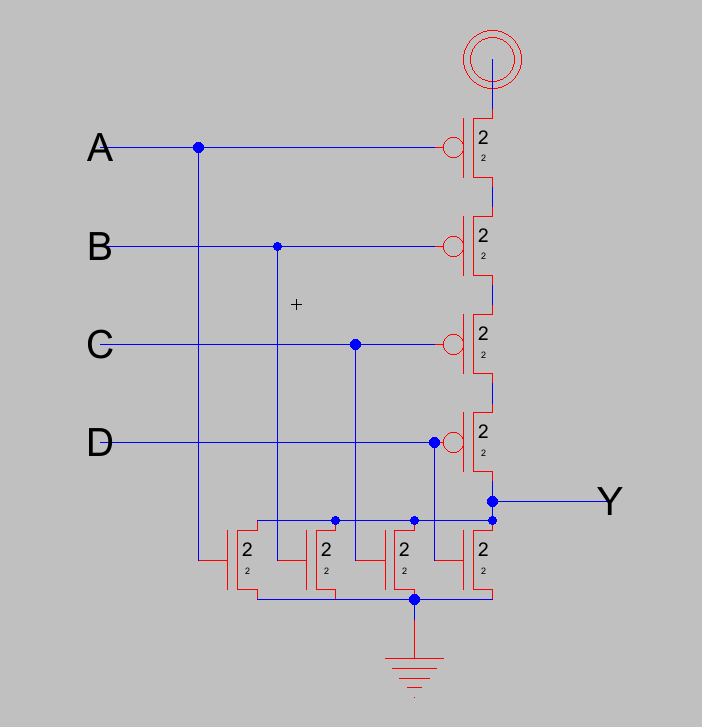
\includegraphics[width=0.4\textwidth]{figures/homework_1-fig_1.png}
		  \caption{NOR4 Schematic}
		  \label{fig:NOR4}
		\end{figure}
	\setcounter{enumi}{5}
	\item
		\begin{enumerate}[label=(\alph*)]
			\item For a gate with the Boolean descriptor \(Y = \overline{ABC + D}\) (AOI31), the pull-down network is first constructed using three series nMOS gates in parallel with a single nMOS gate, and the complementary pull-up network is constructed using three parallel pMOS gates in series with a single pMOS gate.
			\begin{figure}[H]
			  \centering
				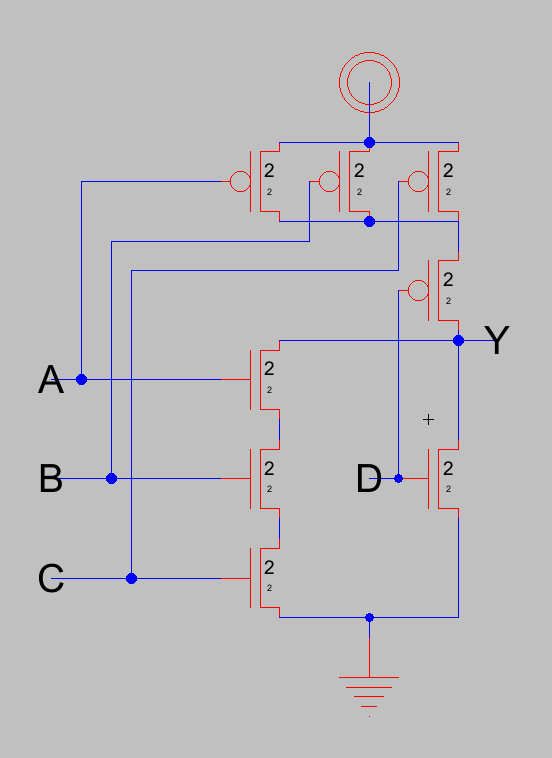
\includegraphics[width=0.4\textwidth]{figures/homework_1-fig_2.png}
			  \caption{AOI31 Schematic}
			  \label{fig:AOI31}
			\end{figure}
		\item For a gate with the Boolean descriptor \(Y = \overline{(AB + C) \cdot D}\), the pull-down network is first constructed using an AOI21 gate in series with a single nMOS transistor, and the complementary pull-up network is constructed with an AOI21 gate in parallel with a single pMOS transistor, which may be simplified into a single AOI21 gate if one of the inputs is considered to be \(AB\).
		\begin{figure}[H]
		  \centering
		  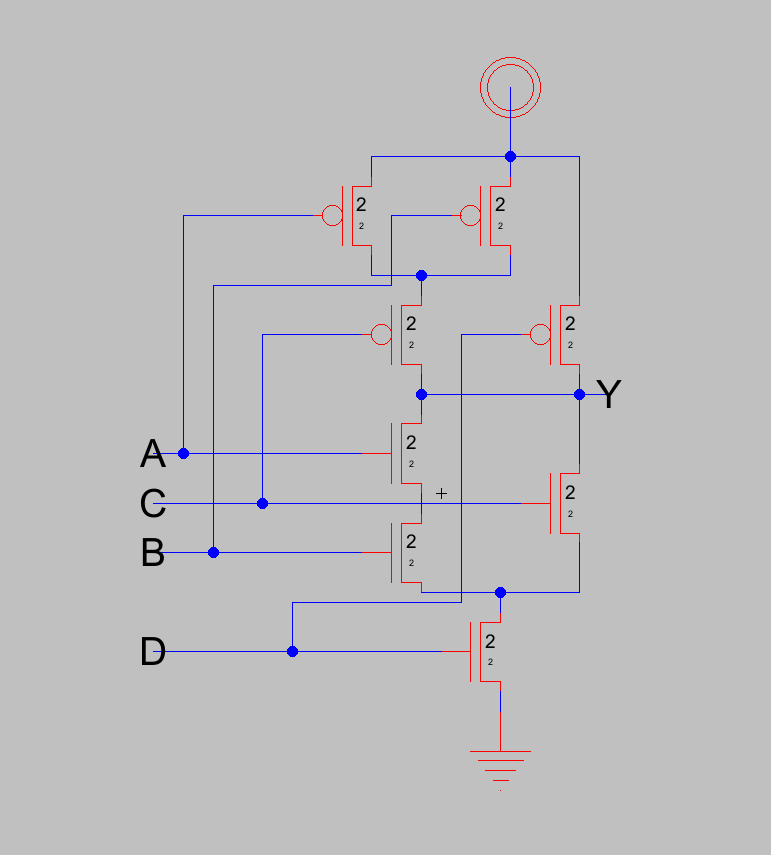
\includegraphics[width=0.4\textwidth]{figures/homework_1-fig_3.png}
		  \caption{AOI21 Schematic}
		  \label{fig:AOI21}
		\end{figure}
	  \item For a gate with the Boolean descriptor \(Y = \overline{AB + C \cdot (A+B)}\), the pull-down network is constructued using a series combination of AOI21 and AOI11 gates, while the pull-up network is constructed using a parallel combination of AOI21 and AOI11 gates, which may be simplified into a single OAI21 gate if one input is considered to be \(AB\) and another is considered to be \(A+B\).
			\begin{figure}[H]
			  \centering
			  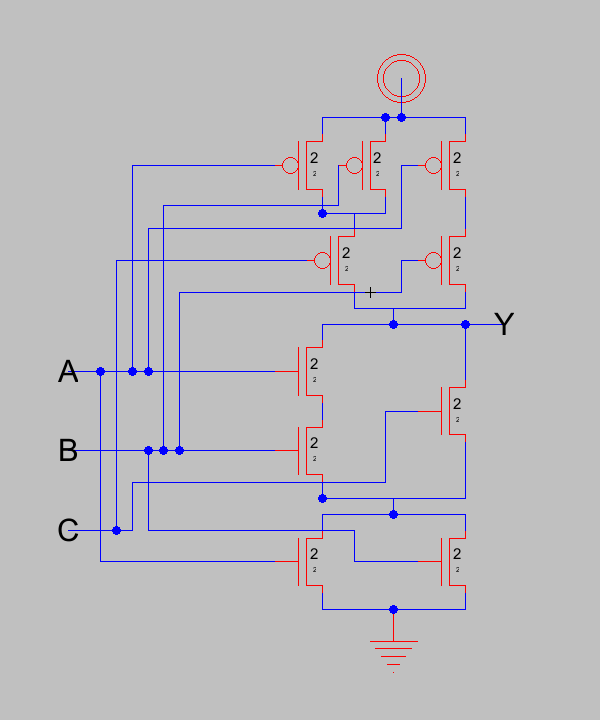
\includegraphics[width=0.4\textwidth]{figures/homework_1-fig_4.png}
			  \caption{OAI21 Schematic}
				\label{fig:OAI21}
			\end{figure}
		\end{enumerate}
	\setcounter{enumi}{9}
	  \item The following is a stick diagram for the 4-input NOR gate seen in Fig. 1:
		\begin{figure}[H]
		  \centering
		  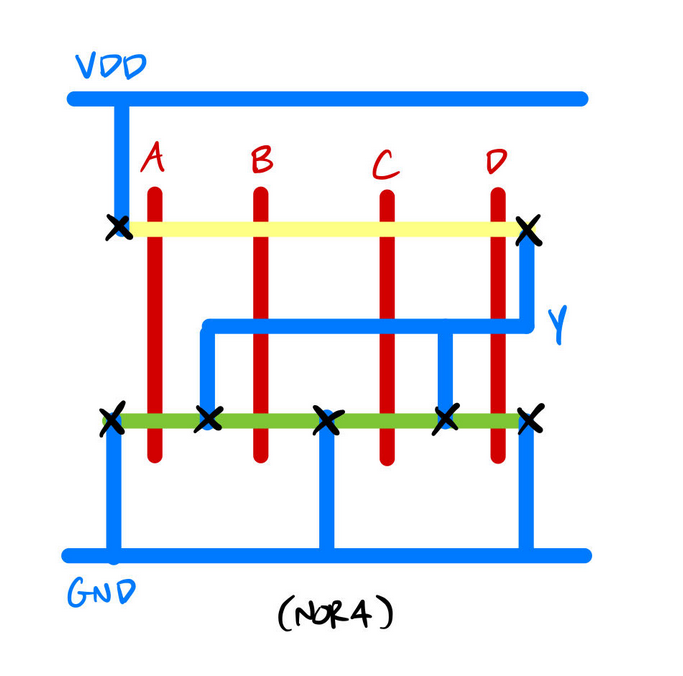
\includegraphics[width=0.6\textwidth]{figures/homework_1-fig_5.png}
		  \caption{NOR4 Stick Diagram}
		  \label{fig:NOR4 Stick}
		\end{figure}
	\setcounter{enumi}{13}
	  \item Estimating the size of the layout shown by the stick diagram in Figure 1.75 of the textbook (Fig. 6), we can count horizontal wiring tracks from top to bottom (4) and vertical tracks from left to right (5), including the clock trace and slightly wider-than-normal space between the two middle connection points (8). Multiplying each by \(8\lambda\), we can estimate the gate's size as \(40\lambda \times 64\lambda\).
    \begin{figure}[H]
      \centering
      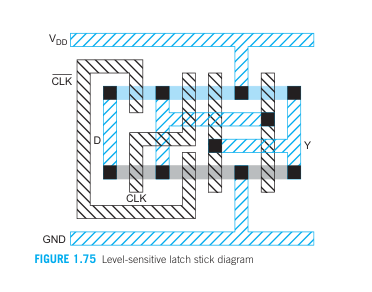
\includegraphics[width=0.8\textwidth]{figures/homework_1-fig_6.png}
      \caption{Textbook Diagram}
      \label{fig:Textbook Diagram}
    \end{figure}
	\setcounter{enumi}{15}
	  \item
		\begin{enumerate}[label=(\alph*)]
			\item For a gate with the Boolean descriptor \(\overline{(A+B)\cdot C}\), the pull-down network is constructed using a parallel combination of nMOS transistors in series with a single nMOS transistor, and the complementary pull-up network is constructed using two series pMOS transistors in parallel with a single pMOS transistor. 
			\begin{figure}[H]
			  \centering
				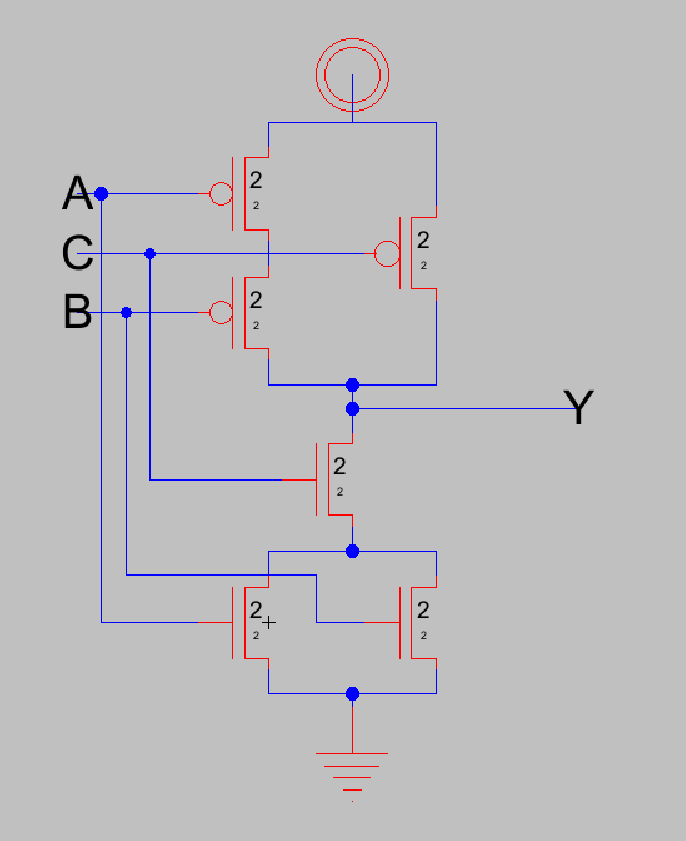
\includegraphics[width=0.4\textwidth]{figures/homework_1-fig_7.png}
			  \caption{OAI21 Schematic}
			  \label{fig:OAI21_2}
			\end{figure}
		\item The following is the corresponding stick diagram: 
		\begin{figure}[H]
		  \centering
		  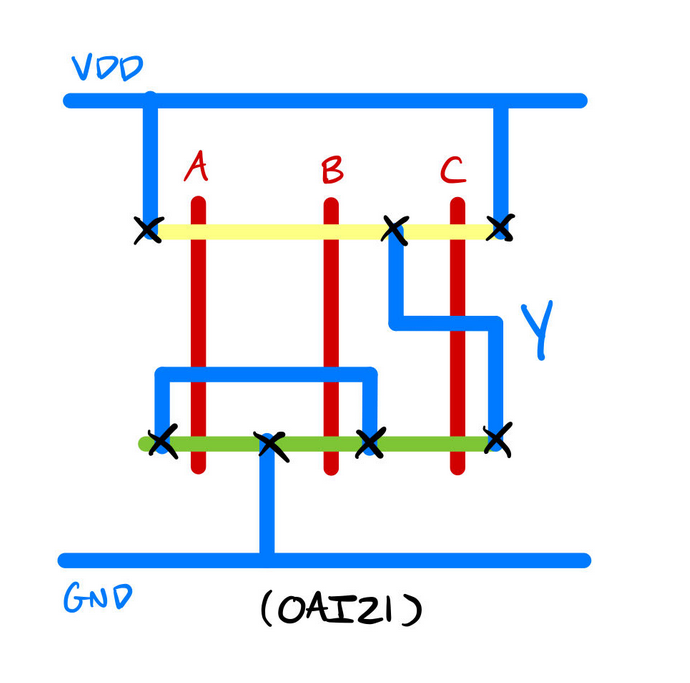
\includegraphics[width=0.6\textwidth]{figures/homework_1-fig_8.png}
		  \caption{OAI21 Stick Diagram}
		  \label{fig:OAI21 Stick}
		\end{figure}
	\item Estimating the size of the layout, again, using vertical and horizontal wiring tracks, we may estimate an area of \(32\lambda \times 32\lambda\).
		\end{enumerate}
\end{enumerate}
\end{document}
